\chapter{Building a Modular Synthesizer}\label{chapter:building-a-mod-synth}

\section{The Modules: Pure Waveforms}

The waveforms created through SuperCollider are through the ``SinOsc'' Unit Generator. As in Listing \ref{lst:sinewave-synthdef}, a simple sine wave is created, with a frequency of 440 Hz ($A_4$, or Concert A), and a volume of 50. Thus, as previously seen in both Figure \ref{fig:basic-sine-wave} and Equation \ref{eq:sine-wave-equation}, a continuous sine wave has been created.

\begin{listing}
	\begin{lstlisting}
		SynthDef("sinewave", {arg freq=440, vol=50; Out.ar(0, SinOsc.ar(freq, 0, vol))}).add;
	\end{lstlisting}
	\caption{Creating a sine wave SynthDef in SuperCollider}
	\label{lst:sinewave-synthdef}
\end{listing}

\begin{listing}
	\begin{lstlisting}
		x = Synth("sinewave");
	\end{lstlisting}
	\caption{Putting the sine wave SynthDef into a Synth, for sound output}
	\label{lst:sinewave-synth}
\end{listing}

\subsection{Volume Slider}

Volume is a simple concept to understand, as it is how loud or soft the human ear hears at a particular frequency. The sine wave SynthDef created in Listing \ref{lst:sinewave-synthdef} contains a variable value for volume. In the SynthDef, the volume is initialized at the number 50, which generally correlates to a medium-loud volume of \textit{mezzo forte}. The variable A of the generic sine wave equation \ref{eq:sine-wave-equation} is equivalent to this change in volume.

As the sine wave Synth Def contains two variables, one for frequency, and one for volume, creating modules for both a volume slider and a pitch knob is simple. To create the volume slider, a SuperCollider class called \textit{EZSlider} creates the outline of the volume slider itself, as in Figure \ref{fig:volume-slider-basic}. For the slider's functionality, there are three important parts: the ``controlSpec,'' ``action,'' and ``initVal.'' The ``controlSpec'' defines the ``control spec,'' or the range of values allowed for the specified module. Negative volume does not exist, so this simple volume module will contain valid values for 0 volume (\textit{pianissimo}) up to 100 volume (\textit{fortissimo}). Then, the ``action'' argument of the \textit{EZSlider} class determines the function that runs when the value of the volume slider is changed. 

\begin{figure}[h]
  \centering
  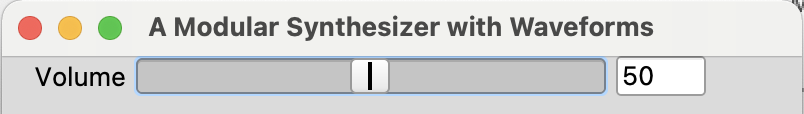
\includegraphics[width=\textwidth]{volume-slider-basic.png}
  \caption{The basic volume slider, with a volume of 50, or \textit{mezzo forte}}
  \label{fig:volume-slider-basic}
\end{figure}

\begin{listing}
	\begin{lstlisting}
		volumeSlider = EZSlider(awindow, label:"Volume", controlSpec:[0,100], action:{|volumeSliderValue| x.set("vol", volumeSliderValue.value)}, initVal:50);
	\end{lstlisting}
	\caption{Creating the volume slider in SuperCollider}
	\label{lst:volume-slider-waveform}
\end{listing}

In Listing \ref{lst:volume-slider-waveform}, the action that is set involves changing the volume of the Synth created in Listing \ref{lst:sinewave-synth}. In this code example, the SynthDef from Listing \ref{lst:sinewave-synthdef} that is assigned to the variable name ``sinewave'' is now put into a Synth. This Synth, as previously described, allows SuperCollider to deal with audio output. So, the SynthDef ``sinewave'' is put into a Synth, known as ``x.'' Within the action, $x$ can be manipulated, that is the sine wave which is in the Synth can be manipulated, resulting in an altered sound. The action itself begins with a reference to the volume slider, $mv$. The Synth, $x$, then references the volume argument from the SynthDef, ``vol,'' which sets the volume for both the SynthDef and the Synth, and uses the \texttt{set} function to set the volume of the Synth equal to the volume that the volume slider contains. The volume of the Synth $x$ will update as the value of the volume slider does, setting the value of \texttt{x.vol} to be equivalent to \texttt{mv.value}. Finally, ``initVal'' simply initializes the starting value of the slider to volume 50 (\textit{mezzo forte}).

\subsection{Pitch Knob: The Pitch Bend}

Pitch, as previously mentioned, is simply a functionality which dictates the frequency of a note that the human ear perceives. Standard Western tuning currently dictates notes to be tuned around the starting pitch of the note A above Middle C (or $A_5$), which is equivalent to 440 Hz.

In Listing \ref{lst:sinewave-synthdef}, we notice that the sine wave SynthDef is created, with two arguments: the frequency for the sine wave to play at, and the volume of the sine wave. The frequency of the sine wave that is created is equivalent to the variable \textit{B} in the generic sine wave equation (Equation \ref{eq:sine-wave-equation}).

Similar to the volume slider, creating the pitch knob in SuperCollider relies on the use of a native class, \textit{EZKnob}. This class creates the knob, as in Figure \ref{fig:pitch-wheel-basic}. Like with the class \textit{EZSlider}, the knob also has the ``controlSpec,'' ``action,'' and ``initVal.'' The controlSpec for the pitch knob is \texttt{freq}, denoting the span of available frequencies, of the valid notes within standard tuning systems. While negative frequency values do not exist, valid frequency values would exist within the human range of hearing (that is, 20 Hz to 20 kHz). The ``action'' argument works similarly to its functionality in the volume slider, as it sets the \texttt{freq} argument of SynthDef ``sinewave'' equal to the frequency value of the pitch knob. Then, the Synth of Listing \ref{lst:sinewave-synth}, ``x,'' continuously matches the value of the pitch knob (\texttt{mn.value}) to the frequency value of the SynthDef, and thus also the Synth. The final argument of the \textit{EZKnob} class is ``initVal,'' in which the initial value of the pitch knob is set to 440 Hz.

\begin{figure}
  \centering
  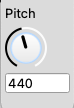
\includegraphics{pitch-wheel-basic.jpg}
  \caption{The basic pitch wheel, with a pitch of 440 Hz, or $A_5$}
  \label{fig:pitch-wheel-basic}
\end{figure}

\begin{listing}
	\begin{lstlisting}
		pitchKnob = EZKnob(awindow, label:"Pitch", controlSpec:\freq, action:{|pitchKnobValue| x.set("freq", pitchKnobValue.value, currentFreq)}, initVal:440);
	\end{lstlisting}
	\caption{Creating the pitch knob in SuperCollider}
	\label{lst:pitch-knob-waveform}
\end{listing}



\subsection{Legato Switch: A Sustain Button}

The \textit{legato} switch for this synthesizer is meant to emulate the \textit{legato} notation found in classical music. \textit{Legato} is a directive, typically found in its full form in classical music, which indicates the performance of a specific passage to be played in a smooth, graceful, and connected style (opposed to the \textit{staccato} notation) \cite{Winer_2018}. It will often be indicated by a slur over the notes, or an accent mark with a line over the notes to be affected, as in Figure \ref{fig:legato-notes-example} \cite{Henle_2009}. On a physical electronic keyboard, this module is most often seen with a \textit{sustain} button, in which the notes played are extended, and slurred into each other. However, it is important to note that not all slur lines in written sheet music will be meant to be played \textit{legato}. Notes that are to be played \textit{legato} will differ in pitch, connecting notes of different pitches to be played in succession in a smooth manner. This is unlike the notation for tied notes, as in Figure \ref{fig:tied-notes-example} \cite{Lung_2016}, which connect notes that are the same pitch. The durations of the notes which are tied together are combined, and played at that new longer note duration instead. However, further development on this module is not needed. A continuous pure sound wave was created through the SynthDef, and later put into a Synth for sound output. A module to sustain a pure tone and smoothly connect it to the next pure waveform will not alter the output sound of the continuous waveforms which are created within SuperCollider code.

\begin{figure}[h]
  \centering
  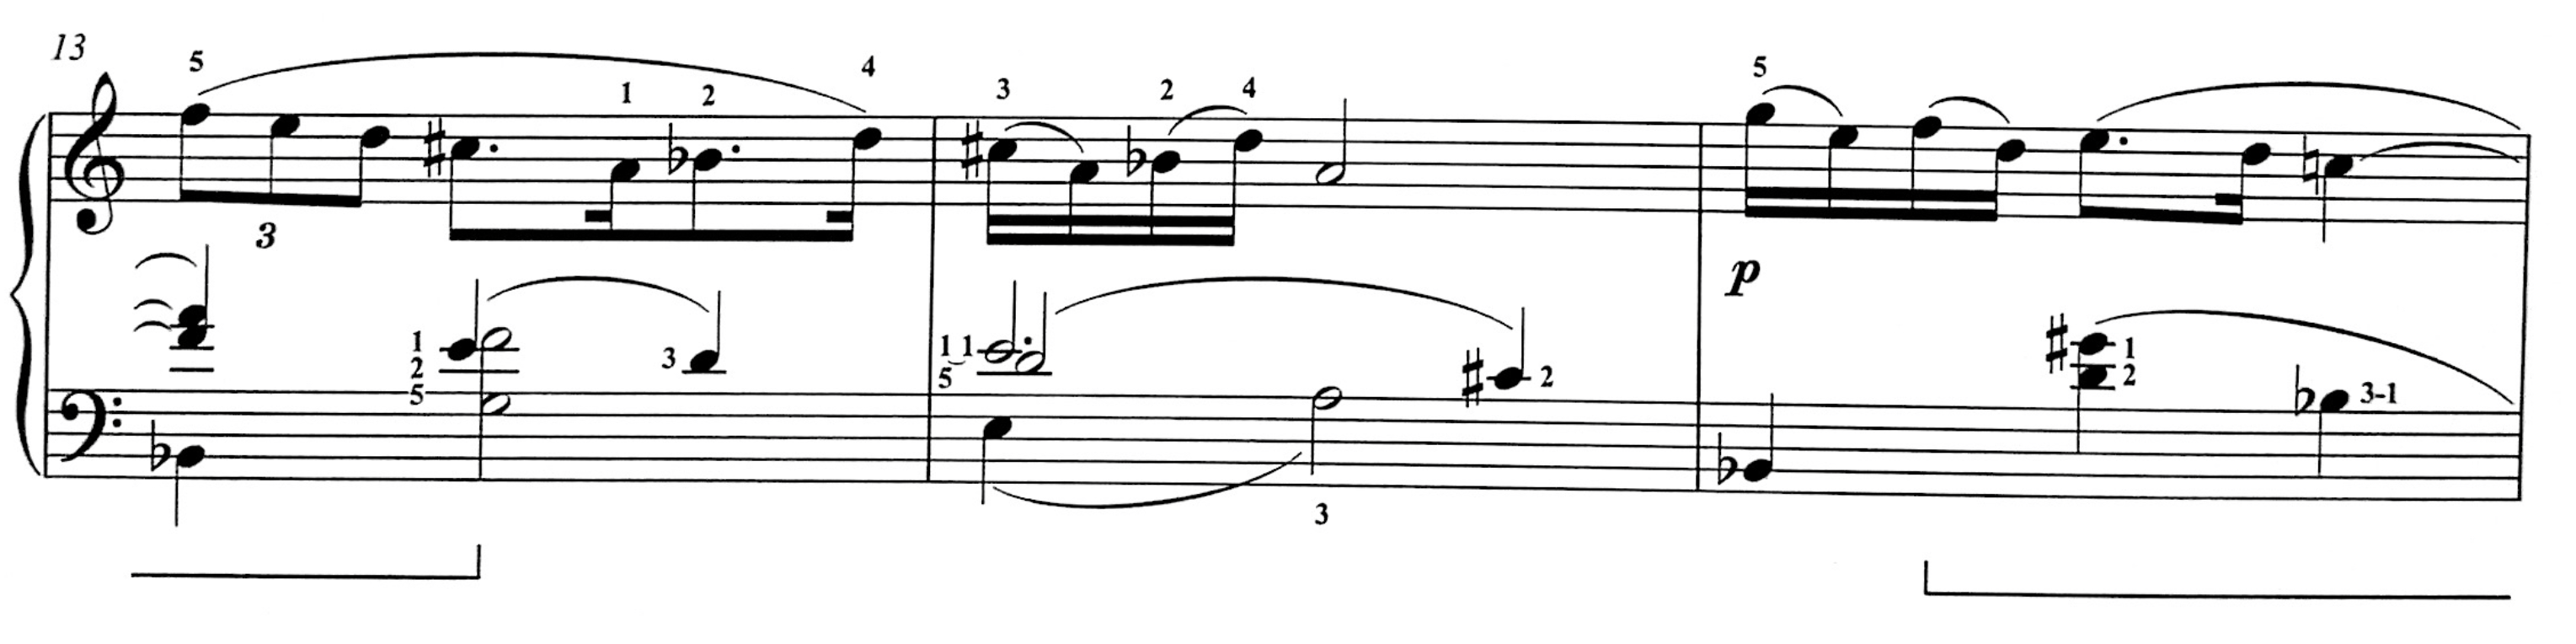
\includegraphics[width=\textwidth]{bartok-dance-four-b-section-second-system.jpg}
  \caption{Béla Bartók, Six Romanian Folk Dances, \textit{Buciumeana},  mm. 13-15}
  \label{fig:legato-notes-example}
\end{figure}

\begin{figure}[h]
  \centering
  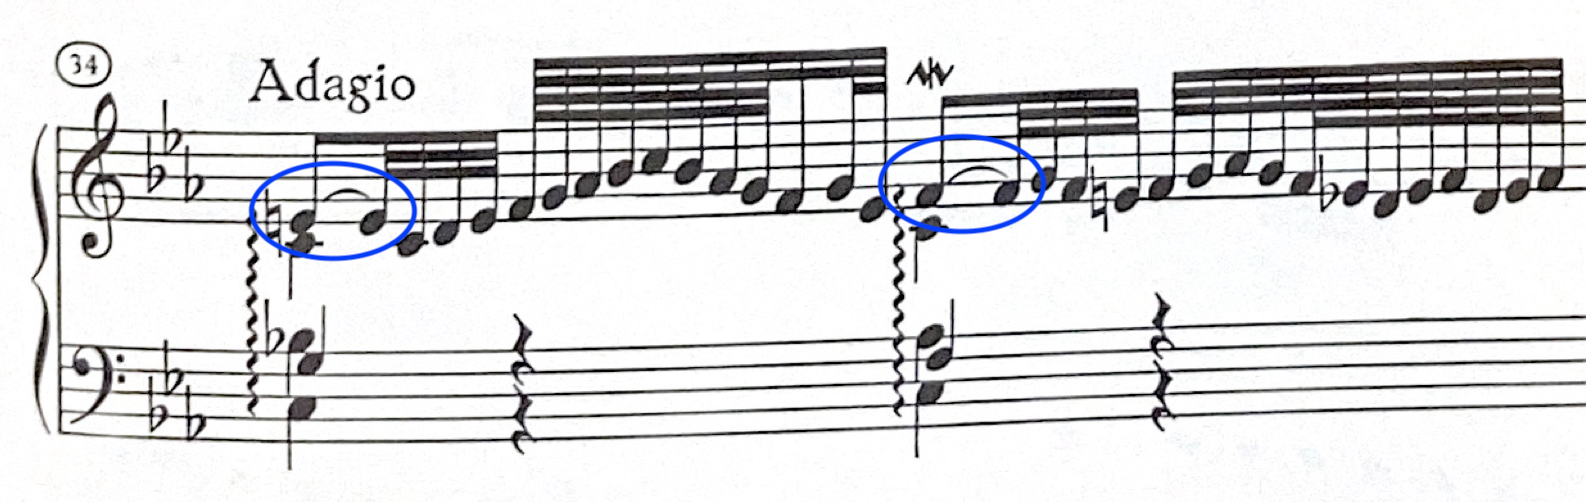
\includegraphics[width=\textwidth]{bach-prelude-second-motive.jpg}
  \caption{Johann Sebastian Bach, The Well-Tempered Clavier Book I, \textit{Prelude in C Minor}, mm. 34-35}
  \label{fig:tied-notes-example}
\end{figure}

\subsection{Major Chord Generator}

The Major Chord Generator within this modular synthesizer involve two pieces: calculating the proper frequencies of the major third and perfect fifth intervals--as they are subject to change from the user's input on the pitch knob--and adding these two intervals to play simultaneously with the original waveform sound. First, to calculate the proper intervals of tonic note to major third, and tonic note to perfect fifth, \textit{interval ratios} (the widths of semitones) are used. As mentioned within Subsection \ref{subsection:how-midi}, the commonly used tuning system in the Western world is the twelve-tone equal temperament system, which divides the octave into 12 parts. Each of these parts are equally tempered (or equally spaced) on a logarithmic scale, such that each ratio is equal to $2^\frac{1}{12}$, or $\sqrt[12]{2} \approx 1.05946$ (the 12th square root of 2, and $a$ in Equation \ref{eq:equal-temperament-eq} \cite{Suits_1998}). This tuning system is normally tuned relative to the standard pitch of 440 Hz, known as \textit{A440}, signifying that the note $A$ (typically $A_4$, or Concert A) is tuned to 440 Hertz, and all other notes are defined relative to this pitch, as some multiple of semitones away from it, either higher or lower in frequency. Thus,  the modular synthesizer created also begins with a starting pitch of A440, every other pitch is defined relative to it ($f_0$ in Equation \ref{eq:equal-temperament-eq}).

Within the twelve-tone equal temperament system, calculating the intervals for the major third and perfect fifth is some multiplication of the single semitone $\sqrt[12]{2}$. As there are four semitones between the tonic note and its major third, the interval ratio is $2^\frac{4}{12}$, or $\sqrt[\frac{4}{12}]{2}$, and seven semitones between the tonic and perfect fifth, the interval ratio is $2^\frac{7}{12}$, or $\sqrt[\frac{7}{12}]{2} \approx \sqrt[12]{128}$, as in Listing \ref{lst:chord-creation} and Equation \ref{eq:equal-temperament-eq}. 

\begin{listing}
	\begin{lstlisting}
		var baseFrequency = 440;
		var thirdFreq = baseFrequency * (2**(4/12));
		var fifthFreq = baseFrequency * (2**(7/12));
	\end{lstlisting}
	\label{lst:chord-creation}
	\caption{Creating the major third and perfect fifth intervals}
\end{listing}

\begin{equation}
	f_n = f_0 * (a)^n
	\label{eq:equal-temperament-eq}
\end{equation}

After calculating the ratio of frequencies, the work on the second part of the module begins. Similar to the work done to create the initial waveform, two additional pure waveforms, and their Synth counterparts, are created (Listing \ref{lst:major-chord-synths}). Then, the only step which remains involves adding the Synths $y$ and $z$ into a variable to play simultaneously (Listing \ref{lst:major-chord-module}) using an array called ``majChord.''

\begin{listing}
	\begin{lstlisting}
		SynthDef("sinewave_third", {arg vol=50; Out.ar(0, SinOsc.ar(thirdFreq, 0, vol))}).add;
		SynthDef("sinewave_fifth", {arg vol=50; Out.ar(0, SinOsc.ar(fifthFreq, 0, vol))}).add;
		y = Synth("sinewave_third");
		z = Synth("sinewave_fifth");
	\end{lstlisting}
	\label{lst:major-chord-synths}
	\caption{Creating SynthDefs for the major third and perfect fifth intervals}	
\end{listing}

\begin{listing}
	\begin{lstlisting}
		majChord = ["sinewave", "sinewave_third", "sinewave_fifth"];
	\end{lstlisting}
	\label{lst:major-chord-module}
	\caption{Combining the three waveform Synths into an array ``majChord''}
\end{listing}

The ``majChord'' variable is placed into a button class \textit{Button}, which has two states, depending on the on/off status of the button itself (Listing \ref{lst:major-chord-button}). Once the button's status is changed to on, all three Synths within the ``majChord'' array will sound at once.

\begin{listing}
	\begin{lstlisting}
		majorChord = Button(awindow, Rect(20, 20, 150, 25)).states_([["Turn Major Chord Off", Color.black, Color.gray], ["Turn Major Chord On", Color.black, Color.yellow]]);	
	\end{lstlisting}
	\label{lst:major-chord-button}
	\caption{Implementing the major chord module using the \textit{Button} class}
\end{listing}

\subsection{Delay Slider}

To create the delay slider, which determines the time which the waveform is delayed, we rely on the same native SuperCollider class we did to create the volume slider: \textit{EZSlider}. Like with the volume slider, we are using the same three arguments: controlSpec, action, and initVal. For the control spec of the delay slider, we must make sure these values match those available in the unit circle, so that the valid range of values is between $\frac{\pi}{6}$ to $\frac{11\pi}{6}$. While it is possible to use values greater than $\frac{11\pi}{6}$, or less than $\frac{\pi}{6}$ in theory, in practice it will sound equivalent to values within this range, as the sine wave will be overlaid directly on top of the possible values in this range. 

\begin{listing}
	\begin{lstlisting}
		delaySlider = EZSlider(awindow, label:"Delay Time", labelHeight:50, labelWidth:100, controlSpec:[(-pi)/6, pi/6], action: {|md| x.set("phase", md.value)}, initVal:0);	
	\end{lstlisting}
	\caption{Creating a delay slider in SuperCollider}
	\label{lst:delay-slider}
\end{listing}

In SuperCollider the time values for delay are calculated in radians, so using the values from the unit circle works well. For the ``action'' argument, similarly to previous modules, the phase of Synth ``x'' is set to be equivalent to the value of the delay slider. The slider itself is initialized to 0, where there is no early or late arrival of the sound.

\subsection{Adding Distortion}

The distortion of a simple pure audio signal involves a SuperCollider class known as \textit{InsideOut}. For this module, both clipping and fuzz are used. As in Listing \ref{lst:distortion-waveforms}, there are two aspects which create the clipping and fuzz effects: a sine wave Unit Generator (UGen), and a \texttt{Pink Noise} UGen. The sine wave UGen allows for the clipping of the sound wave. The \texttt{Pink Noise} UGen is added through the fuzz effect, using the value 30 as the frequency multiplier, and allows us to add a type of colored noise known as ``pink noise.''

\begin{listing}
	\begin{lstlisting}
		// PinkNoise function, with a sine wave UGen at the frequency from pitchKnob
		dist = {InsideOut.ar(SinOsc.ar(baseFrequency) + PinkNoise.ar(0.9, 0), 30, 50)}.scope;
	\end{lstlisting}
	\caption{Creating a distortion module}
	\label{lst:distortion-waveforms}
\end{listing}

Pink noise is used as it is a type of noise which contains all the possible frequencies which a human can hear. Unlike other types of colored noise, pink noise is much less intense. There are multiple types of colored noise, including black, red, blue, brown, and white. However, for music production, the two most popular types of colored noise are white noise and pink noise. White noise operates similarly to white light, encompassing the entire frequency of audible sound from low pitches to high pitches equally. Different frequencies are played randomly across the entire audible range, and normally sounds like radio static \cite{Unison_2021}. When mixing white noise into a pre-existing music mix, white noise fills sonic space similar to how low bass notes fill sonic space in the very low end (refer to Table \ref{tbl:frequency-table-of-human-hearing-general}). Pink noise is very similar to white noise, but constructed differently. It creates equal amplitudes based on the octaves, getting softer and less abrasive-sounding as the pitch rises. Thus, lower frequencies are louder, and higher frequencies are easier to listen to and are softer \cite{Unison_2021}. As it technically has a fundamental frequency, it will sound much more natural than white noise, as natural sounds all have a specific fundamental frequency (defined as the lowest harmonic played).

\section{MIDI Input}\label{section:midi-input}

Input with MIDI in SuperCollider is more complex than creating pure sound waveforms for modular changes; however there are some similarities, we must create three aspects for modular sound synthesis: the \texttt{Synth}, \texttt{SynthDef}, and MIDI functions for MIDI itself to be able to output sound. 

Before any of this, however, the MIDI inputs and the MIDI client must be initialized. As in Listing \ref{lst:initialize-midi}, there are two key steps to using MIDI in SuperCollider: initializing the MIDI client and connecting to the specific MIDI controller that will be used. Once this is done, we can move on to creating the MIDI functionality itself.

\begin{listing}
	\begin{lstlisting}
		MIDIClient.init;
		MIDIIn.connect;
	\end{lstlisting}
	\caption{Initializing the MIDI Client}
	\label{lst:initialize-midi}
\end{listing}

Creating a SynthDef for MIDI input will be the easiest task. To create a SynthDef for MIDI use, we do what is in Listing \ref{lst:midi-synthdef}. 

\begin{listing}
	\begin{lstlisting}
		SynthDef("piano", {arg freq = 440, amp = 0.1, gate = 1;
		var snd, env;
		env = Env.adsr(aLevel, dLevel, sLevel, rTime, amp).kr(2, gate);
		snd = Saw.ar(freq: [freq, freq*1.5], mul: env);
		Out.ar(0, snd)
		}).add;
	\end{lstlisting}
	\caption{Creating a MIDI SynthDef with a ADSR envelope}
	\label{lst:midi-synthdef}	
\end{listing}

Listing \ref{lst:midi-synthdef} describes the necessary aspect in the creation of a SynthDef that will  be compatible with MIDI commands. The ADSR envelope, or ``envelope generator'' (a term which refers to the ``shape'' of a sound, or the contour by which a sound gets louder and softer) is described by its stages: Attack, Decay, Sustain, Release, as in Figure \ref{fig:adsr-envelope} \cite{Puckette_2007}. Some of this was discussed in the Note On and Note Off messages subsections of Section \ref{section:midi-messages}. The order in which sound goes through an envelope generator is important, as sound must travel through the attack, decay, sustain, and release stages in that order, and is unable to go back to any other stage once it comes to a stage. An ADSR envelope generator will first receive a gate input, the variable \texttt{gate}, and raise the value of \texttt{gate} to the maximum volume or voltage (if we were to use a physical envelope generator within an analog synthesizer) the envelope generator is able to output, or the output level that is set over a specific time by the Attack control. The gate is one of the main signal types of a modular synthesizer. It will jump from a base level (normally 0) to a higher one when a new note is meant to start, such as when a user presses down on a MIDI keyboard, or another transition is meant to happen, such as when the next stage of the ADSR envelope is meant to start. When a user presses down on a MIDI keyboard, the gate will typically stay at the level it was given for the duration of that note, and then suddenly drop to its baseline level once the key is released. Thus, when the \texttt{gate} variable is sent through a typical envelope generator like the ADSR envelope generator, the beginning of the gate increases to its maximum volume as it tells the envelope to go through the Attack and Decay stages. As the gate remains at this high level, the envelope may go into the Sustain stage, and then when the gate's volume returns to its baseline level, the envelope will move into the Release stage. 

\begin{figure}
  \centering
  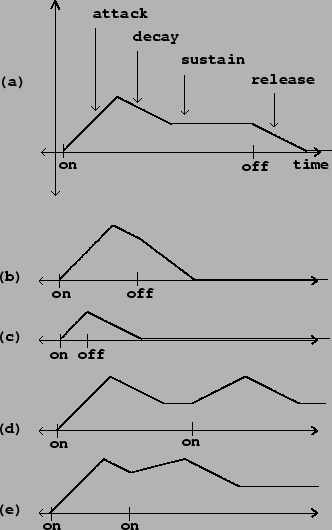
\includegraphics[width=0.4\textwidth]{adsr_envelope.png}
  \caption{ADSR envelope output: (a) with ``on" and ``off" triggers separated; (b) and (c) with early ``off" trigger; (d), (e) re-attacked.} \cite{Puckette_2007}
  \label{fig:adsr-envelope}
\end{figure}

Once the sound reaches this defined high level of the Attack stage, the Decay control will cause the sound to begin dropping in volume, until it reaches the volume set by the Sustain control. If the \texttt{gate} variable is still active (and has a value other than 0), the level set by the Sustain control is maintained until the value of \texttt{gate} returns to 0--which typically signifies the user has released the key on a compatible keyboard or controller. When \texttt{gate} is no longer active, the output volume begins to drop back to a volume of 0, in which the rate of this drop is determined by the Release control. 

A key concept to understanding the ADSR envelope is that there is a difference in behavior when the ADSR envelope is not able to finish the entire four-stage cycle. If the user were to release the key before the Attack or Decay stages finish, then the envelope may skip to the Release stage, passing over the Sustain control entirely, and continuing to the Release control with the current volume level. However, if the user were to re-trigger the envelope by sending a new \texttt{gate} through to the synthesizer, a digital envelope generator will return the volume level back to 0, and restart the envelope cycle.

Other arguments within the SynthDef of Listing \ref{lst:midi-synthdef} include \texttt{freq}, and \texttt{amp}, which will help in modifying the input MIDI key presses. Creating the Synth and MIDI functions for proper MIDI functionality are much more difficult. When creating the waveform modules, there was no need to develop functionality for the waveforms, as they were a native aspect of SuperCollider. Within the MIDI modules, creating the Synth and MIDI functions must be done simultaneously. As in Listing \ref{lst:midi-note-on-and-off}, the two primary MIDI messages that will be used are note on and note off. To create a Synth using the ``piano'' SynthDef from Listing \ref{lst:instantiate-synthedef}, it will be wrapped within the SuperCollider MIDI function for note on: \texttt{MIDIdef.noteOn}. With the proper MIDI functionality created, similar modules to those developed for pure waveforms can be made.

\begin{listing}
	\begin{lstlisting}
		on = MIDIdef.noteOn(\keyDown, {arg vel, note, vol;
				notesArray[note] = Synth("piano", [\freq, note.midicps, \amp, vel.linlin(aLevel, dLevel, sLevel, rTime)]);
			});

		off = MIDIdef.noteOff(\keyUp, {arg vel, note;
				notesArray[note].set(\gate, 0);
			});
	\end{lstlisting}
	\caption{Creating MIDI note on and MIDI note off messages}
	\label{lst:midi-note-on-and-off}	
\end{listing}


\section{The Modules: In Midi}\label{section:the-modules-midi}

Within SuperCollider, the \texttt{Env} class supports the creation of an ADSR envelope, which will allow us to create the modules for the MIDI controller. As in Listing \ref{lst:template-adsr-envelope}  \cite{McCartney_2021}, SuperCollider has native functionality for an ADSR envelope. The first four arguments of the \texttt{ADSR} envelope are consistent as we create the maximum levels for the Attack, Decay, Sustain, and Release stages. The other variable which we are interested in is \texttt{peakLevel}, which in this project is known as \texttt{amp}. This variable is different from \texttt{gate}, as seen in Listing \ref{lst:midi-synthdef}. The \texttt{gate} variable helps determine the current active stage of the ADSR envelope, helping sound move through the envelope one stage at a time. The \texttt{amp} variable on the other hand defines the peak level of each of the stages itself. It is the defining high level of the Attack Stage. Through changing the levels of the Attack, Decay, Sustain, and Release stages, we can modify the input sound from a MIDI controller. 

\begin{listing}
	\begin{lstlisting}
		Env.adsr(attackTime: 0.01, decayTime: 0.3, sustainLevel: 0.5, releaseTime: 1.0, peakLevel: 1.0, curve: -4.0, bias: 0.0)
	\end{lstlisting}	
	\caption{Template for creating an ADSR envelope in SuperCollider}
	\label{lst:template-adsr-envelope}
\end{listing}


\subsection{Volume Slider}

The first module of the MIDI synthesizer, the ``volume'' slider, is a misnomer. While the result is the same, and the output sound from the MIDI controller has a different dynamic level, the logic of the module is different from that of the volume slider within the waveform synthesizer. As mentioned, the \texttt{amp} variable determines the peak level of a MIDI note within an ADSR envelope. Thus, the manipulation of \texttt{amp} is important to adjusting the output volume heard by the user. To then create this amp slider, the SuperCollider class \textit{EZSlider} creates the amp slider, with three arguments: ``controlSpec,'' ``action,'' and ``initVal.'' The control spec for this slider is the same as the volume slider for the waveforms, and cannot be negative, as both negative volume and thus a negative amp value does not exist. Valid values of the control spec is thus between 0.1 and 1, the typical range for an \texttt{amp} value. Then the ``action'' of the slider will determine the volume output of the MIDI input. 

\begin{listing}
	\begin{lstlisting}
		ampSlider = EZSlider(awindow, label:"Amp Volume", labelHeight: 100, labelWidth: 150, controlSpec: ControlSpec(0.1, 1, \lin), action:{|ampSliderValue| note.set(\amp, ampSliderValue.value)}, initVal:0.3);
	\end{lstlisting}	
	\caption{Creating the amp slider for MIDI}
	\label{lst:midi-amp-slider}
\end{listing}

In Listing \ref{lst:midi-amp-slider}, the ``action'' involves altering the input signal from a MIDI controller. The \texttt{note} which holds the information for each note on message is accessed, and the value of the \texttt{note}'s \texttt{amp} is set to be equivalent to the slider's value. The \texttt{amp} value will not continuously update itself, a difference from the volume slider. This difference in functionality is due to the nature of both pure sound waveforms and MIDI signal inputs. Within pure sound waveforms, the signal is continuous, and continues to sound until an external force stops the signal. MIDI signals, on the other hand, rely primarily on the usage of note on and note off messages to send sound to a tool which can properly output it. Thus, the \texttt{amp} of the MIDI note on message of Listing \ref{lst:midi-note-on-and-off} will only update when a new MIDI note on message is sent. Finally, the initial value of the slider is at a \textit{mezzo forte} value of 0.3.

\subsection{Major Chord Generator}

A major chord generator for MIDI will create a major chord, and sound two additional frequencies on top of a MIDI note which a user plays. This will create a triadic chord, with two intervals from the base MIDI note: the major third, and the perfect fifth. The major third interval spans four degrees of the diatonic scale within equal temperament, and the perfect fifth spans seven. As with the major chord generator which was built for pure sound waveforms, the major chord generator for MIDI involves the same two aspects: calculating the proper interval frequencies for the major third and perfect fifth interval, and pushing these two intervals to the SuperCollider server \textit{scsynth}. Using Equation \ref{eq:equal-temperament-eq} and the code from Listing \ref{lst:chord-creation}, we understand that the interval of a major third will have a frequency of $440 * 2^\frac{4}{12}$ and the perfect fifth a frequency of $440 * 2^\frac{7}{12}$.

Thus, having already created the proper intervals for the module, we then must push the intervals to play on \textit{scsynth}. This is different from creating this module for pure waveforms in that we no longer must put the major third and perfect fifth intervals into an array for playback. The SynthDef for MIDI is contained within an ADSR envelope, which has more modularity and independence than pure sound waveforms. Thus, we wrap both the variable for the major third interval (\texttt{thirdInterval}) and the perfect fifth interval (\texttt{fifthInterval}) into variables titled \texttt{thirdIntervalSynth} and \texttt{fifthIntervalSynth} respectively. These variables utilize similar logic to the implementation of \texttt{MIDIdef.noteOn}, layering the intervals on top of the user input.

\begin{listing}
	\begin{lstlisting}
		thirdIntervalSynth = Synth("piano", [\freq, thirdInterval, \amp, vel.linlin(0, 127, 0, 1)]);
		fifthIntervalSynth = Synth("piano", [\freq, fifthInterval, \amp, vel.linlin(0, 127, 0, 1)]);
	\end{lstlisting}
	\label{lst:midi-maj-chord}
	\caption{Creating a major chord in MIDI}
\end{listing}

\subsection{Adding Staccato}

The staccato and legato buttons for the MIDI synthesizer are similar. For this module, we rely heavily on two aspects of the ADSR envelope, the Attack level, and the Decay level. In combination, a shorter attack time and a shorter decay time will create a sudden perceived drop in the volume level of a MIDI input signal. As in Listing \ref{lst:midi-note-on-and-off}, we have created four variables which contain the values for each of the four stages of the ADSR envelope: \texttt{aLevel} for Attack, \texttt{dLevel} for Decay, \texttt{sLevel} for Sustain, and \texttt{rTime} for Release. For this module, the values for \texttt{aLevel} and \texttt{dLevel} are set to 0. With Attack set to 0, the sound of the MIDI input will hit immediately after the signal is begun. Decay set to 0 results in no time for the sound's level to fall from its peak of \texttt{amp} to the \texttt{dLevel}.

\subsection{Adding Legato}

The legato button emulates the musical concept of legato. On a physical MIDI keyboard, a legato button will more often be referenced as a \textit{sustain} button, in which the lengths of notes are extended, and flow into one another. For the concept of legato, it is imperative that each note meant to be played legato are of different pitches. If the pitches of notes meant to be played legato are the same, the duration of these notes will simply be elongated--and the notes tied together--to be the sum of each individual note. Two other aspects of the ADSR envelope are important to extend the sounding of a MIDI note, and to connect it to another MIDI note: Attack and Release. As mentioned, increasing the level of the Attack stage will result in the sound of a MIDI input signal lengthening. This results in more time needing to pass before the gate will move onto the second stage of the ADSR envelope. Extending the time the gate is in the Release stage is also important. For proper legato within MIDI, the Release stage will need to be extended, as the ADSR envelope is only within the note on MIDI message. The note within the MIDI note on message will continue to sound, even after the MIDI note off message is sent through SuperCollider.


\subsection{Distortion}

Distortion, the altering and deforming of an audio signal's waveform, is done to add specific textures and harmonic over what an instrumentalist would play. For this module, we add regular distortion to the input MIDI signal, to add additional harmonics. Regular distortion is the easiest type of distortion to implement for MIDI, as it is similar to how distortion would be added in rock music, and guitar solos, with Jimi Hendrix songs as one example. Distortion in this module will be a kind of gentle distortion in which two pure sound waveforms are added on top of the MIDI signal, when a note on message is sent. 

This module is built differently than the distortion module for pure sound waveforms. With pure sound waveforms, we used simple unit waves--such as sine waves and sawtooth waves--and altered the sound through a native SuperCollider class. The pure sound waves were only ever able to output one frequency at a time, a limitation which does not hold true with MIDI. MIDI can output multiple frequencies at once, through the use of multiple note on messages. So it is much easier to simply add pink noise to a sine wave, at the same frequency as the wave which the user is playing, and run that aggregated sound through a class. With MIDI, though we are also adding additional harmonics over an input MIDI signal, we are not adding colored noise. Instead, as in Listing \ref{lst:midi-distortion}, we borrow some logic from the major chord generator, but use a tritone interval instead of the pleasant-sounding major third and perfect fifth intervals. In place of these two intervals, the tritone interval is used. 

The tritone is the interval of an augmented fourth,\footnote{Enharmonically equivalent to the diminished fifth, both the augmented fourth interval and the diminished fifth interval will sound the same to a listener, but are notated differently.} and in the Medieval era of music was known to be the ``devil in music'' or the ``devil's interval'' because it is the most dissonant interval in the diatonic scale. The diatonic scale is the type of scale which we have discussed, and defined as the scale which contains five whole tones and two semitones \cite{Burkholder_Grout_Palisca_2014}. The major and natural minor scales are diatonic in nature, with the semitones falling between the third and fourth tones in the major scale, and the seventh and eighth tones. In C Major, these semitones would fall between the notes E-F (scale degrees three and four), and notes B-C (scale degrees seven and eight). The minor scale is slightly different, with semitones falling between the second and third scale degrees, and the fifth and sixth degrees. In A Minor, these semitones occur between C-D (degrees three and four), and E-F (degrees five and six).

The tritone is made up of six semitones, and is the interval between C and F\musSharp{}, for example. Its unpleasant sound to the human ear can be traced back to a phenomenon found within the human brain: it is hardwired to find harmony and symmetry within music, and is resistant towards dissonant sounds (rather than pleasing consonant sounds). Intervals which sound pleasing to the human ear are those in which there is a simple ratio between the frequencies. This is clear in the ratios of very pleasant intervals: the octave, which contains the very pleasing 2:1 ratio, and the perfect fifth, which has a ratio of 3:2 \cite{Gann}. These frequency intervals continue through the remaining notes of the scale, oscillating between consonant and dissonant intervals. The tritone, as the most dissonant of all the intervals on the diatonic scale, contains a frequency ratio of 45:32 (or 64:45, depending on the tuning method). 

Distortion for MIDI is not meant to sound as pleasing as adding additional harmonics to an electric guitar signal through an amplifier may be. Instead, for the purposes of this module, the tritone interval is used, to give the distortion an unpleasing effect. The distortion effect is also used for this module, albeit in the simple way of adding two pure sound waveforms over the input MIDI signal. As the tritone interval is six semitones away from a root note, we first calculate the tritone interval to be $f_n = 440 * 2^\frac{6}{12}$, using Concert A as the base frequency. Then, as in Listing \ref{lst:midi-distortion}, the tritone frequency is added to two waveform UGens, \texttt{SinOsc} and \texttt{Saw}, which will add the necessary unpleasant sounds to the MIDI input note's frequency.

\begin{listing}
	\begin{lstlisting}
		tritone = baseFrequency * (2**(6/12));
			
		SynthDef("distortionSynthDef", {arg out = 0;
			Out.ar(out, SinOsc.ar(tritone, 0, 50), Saw.ar(tritone, 0, 50))
		}).add;
	\end{lstlisting}
	\caption{Adding distortion in MIDI}
	\label{lst:midi-distortion}
\end{listing}


\subsection{Manually Adjusting the ADSR Envelope}

The final module for the MIDI synthesizer will be a method of manually adjusting the values for the four pieces of the ADSR envelope. The first five modules of the MIDI synthesizer are ``presets,'' (also known as a ``patch'') or pre-defined modules which are pre-programmed into the synthesizer. These presets, which are also found as all five modules in the pure sound waveform version of the synthesizer, allow a user to understand how an output sound may be changed, without requiring a more in-depth understanding of waveforms or ADSR envelopes. Presets found within a synthesizer are typically modules built to function in a particular way, such that a certain effect can be used to a specified degree. Each synthesizer contains ``parameters'' (like with this modular synthesizer in its ADSR envelope) which allow a user to shape a sound, altering the sound depending on how a user may press, hold, and release keys of a controller. Thus, presets are best understood to be a ``snapshot'' of these parameters (the level of Attack, Decay, Sustain, and Release) at specified values.

The easiest method used to alter the levels of Attack, Decay, Sustain, and Release will be through the SuperCollider class \textit{EZKnob}. This knob class allows for small changes in the value of a variable, and for more flexibility than a simple button may allow. This results in the ability of a user to change the sound of an ADSR envelope to their liking, and can even manually replicate the results of the five other modules, as in Figure \ref{fig:adsr-knobs}. To create the four knobs of Figure \ref{fig:adsr-knobs}, we use the \textit{EZKnob} class four times, once per each knob. Each knob will have the same logic, only affecting different aspects of the ADSR envelope, and with a different initial value to the knob, as in Listing \ref{lst:midi-adsr-manual}. The knob which controls Release will have a larger control spec than the three other stages of the envelope, as we have set the value of Release to be larger within the legato module, to make the legato of MIDI inputs clear.

\begin{figure}[h]
  \centering
  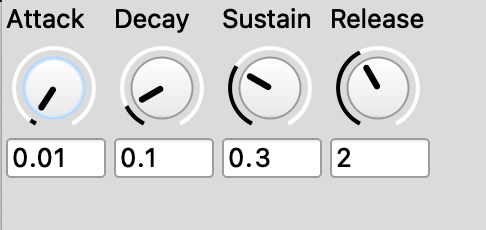
\includegraphics[width=0.4\textwidth]{adsr_knobs.png}
  \caption{The ADSR knobs}
  \label{fig:adsr-knobs}
\end{figure}


\begin{listing}
	\begin{lstlisting}
		attackKnob = EZKnob(awindow, label: "Attack", controlSpec: [0, 1], action:{|attackKnobValue| aLevel = attackKnobValue.value}, initVal: 0.01);

		decayKnob = EZKnob(awindow, label: "Decay", controlSpec: [0, 1], action:{|decayKnobValue| dLevel = decayKnobValue.value}, initVal: 0.1);

		sustainKnob = EZKnob(awindow, label: "Sustain", controlSpec: [0, 1], action:{|sustainKnobValue| sLevel = sustainKnobValue.value}, initVal: 0.3);

		releaseKnob = EZKnob(awindow, label: "Release", controlSpec: [0, 5], action:{|releaseKnobValue| rTime = releaseKnobValue.value}, initVal: 2);
	\end{lstlisting}	
	\caption{Manually adjusting the values of an ADSR envelope}
	\label{lst:midi-adsr-manual}
\end{listing}

As stated, the ability to manually adjust the values for the four stages of the ADSR envelope will allow for greater flexibility, over the pre-programmed values within the other modules of the synthesizer. The combinations of increasing or decreasing the four values will result in different sounds, such that different instruments will appear to have resulted from the alterations. The values for the ADSR envelope which we create in the beginning, in Listing \ref{lst:template-adsr-envelope}, create a sound similar to that of a piano. A piano has a low Attack value, a short Decay time, a relatively medium length but low amp level Sustain, and a short Release time. Other instrument and sound examples, like in Figure \ref{fig:adsr-examples} \cite{Swisher_2019}, are also possible. By setting the Attack and Decay values to be in the middle of the control spec, and Sustain and Release close to 0, a sound similar to that of a kick drum and snare drum is achieved. To create a sound similar to that of a bass guitar or upright bass, set the Decay and Sustain values to be in the middle of the control spec or high, and Attack and Release values to be low. Increasing the level of Attack also will emphasize the initial ``hit'' of the MIDI note on message, causing the sound to appear to be closer. Within music production, this sound would appear to have emphasized the highs and mids (roughly 500 Hz to 4 kHz), and it would become more prominent in a mix. The same is true on the flip side, in which turning down the Attack will make the sound seem to be further away, and give the overall sound more ``space'' and a bigger soundstage. This is best seen in rhythm guitars and bass guitars and upright bass, in which the sound is needed, but should not be a prominent part of a mix. The other method of creating a larger soundstage within the ADSR envelope and a mix is to increase the level of Sustain, as if the microphone used to record the instrument was placed further away. 

\begin{figure}
  \centering
  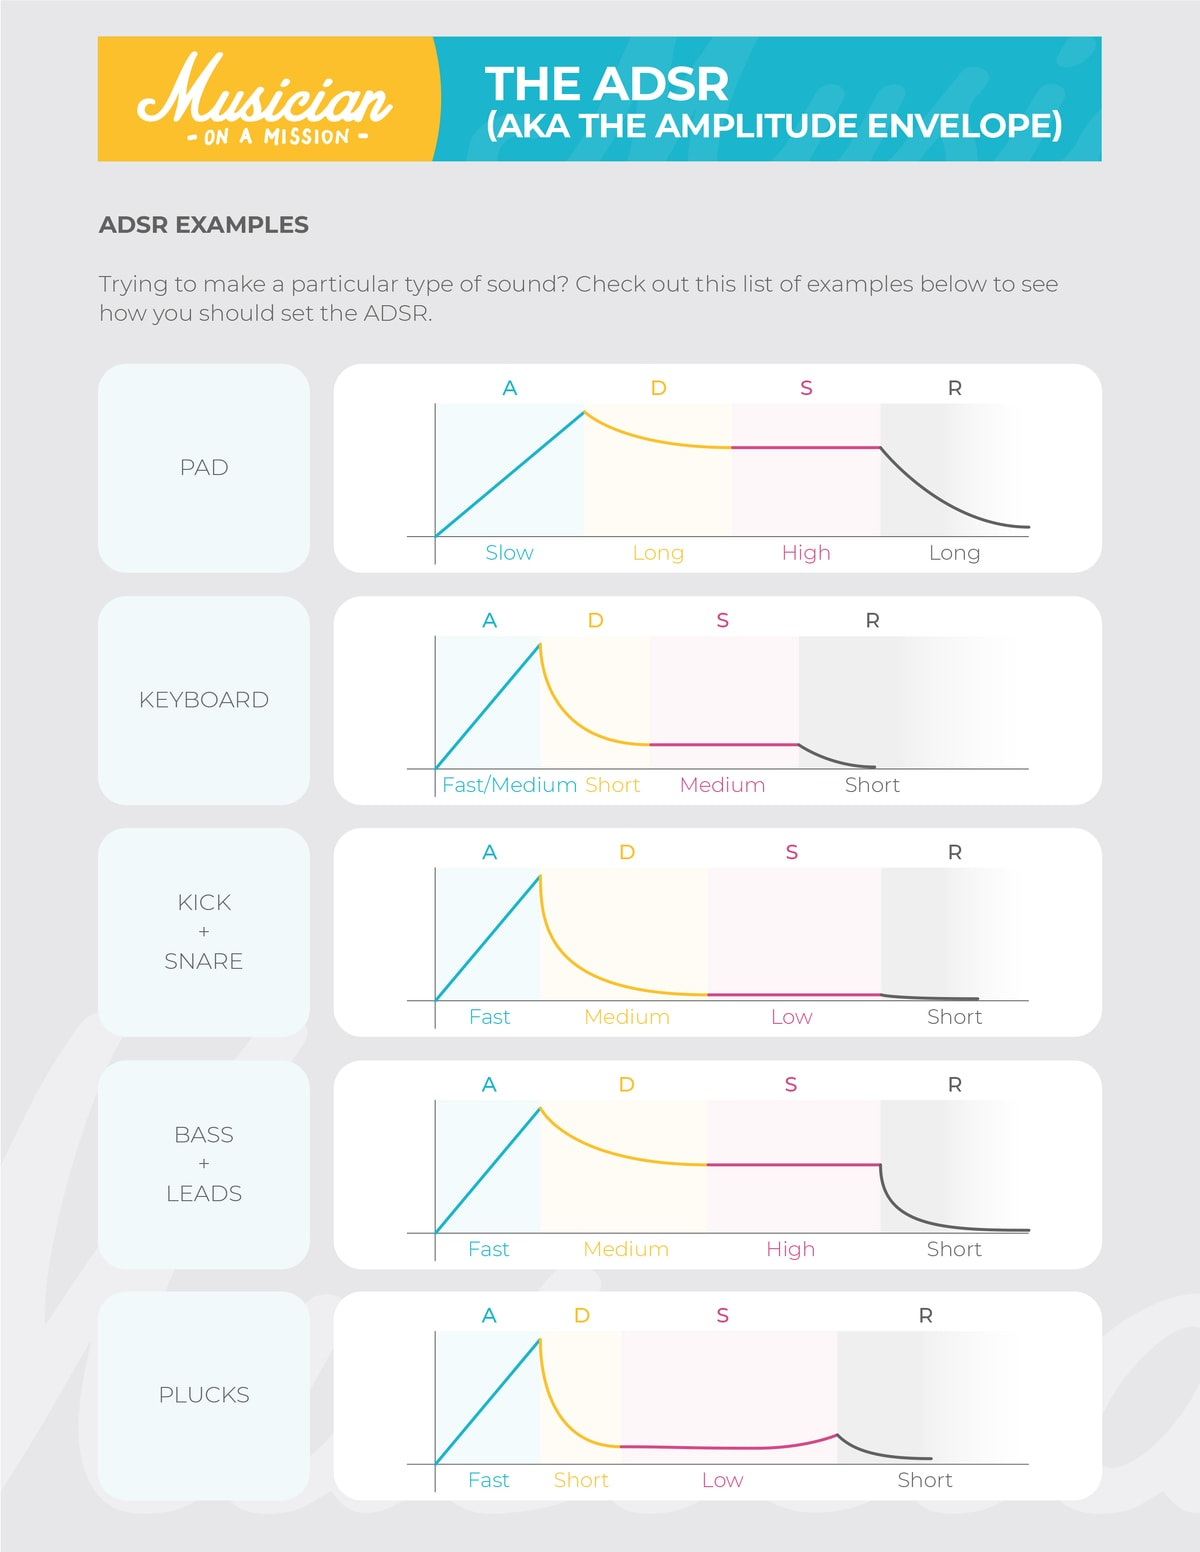
\includegraphics[width=0.4\textwidth]{adsr_examples.jpeg}
  \caption{Other examples of ADSR values} \cite{Swisher_2019}
  \label{fig:adsr-examples}
\end{figure}
